\section{Simulated serological data from \texttt{serosim}}

\begin{figure}[h]
    \centering
    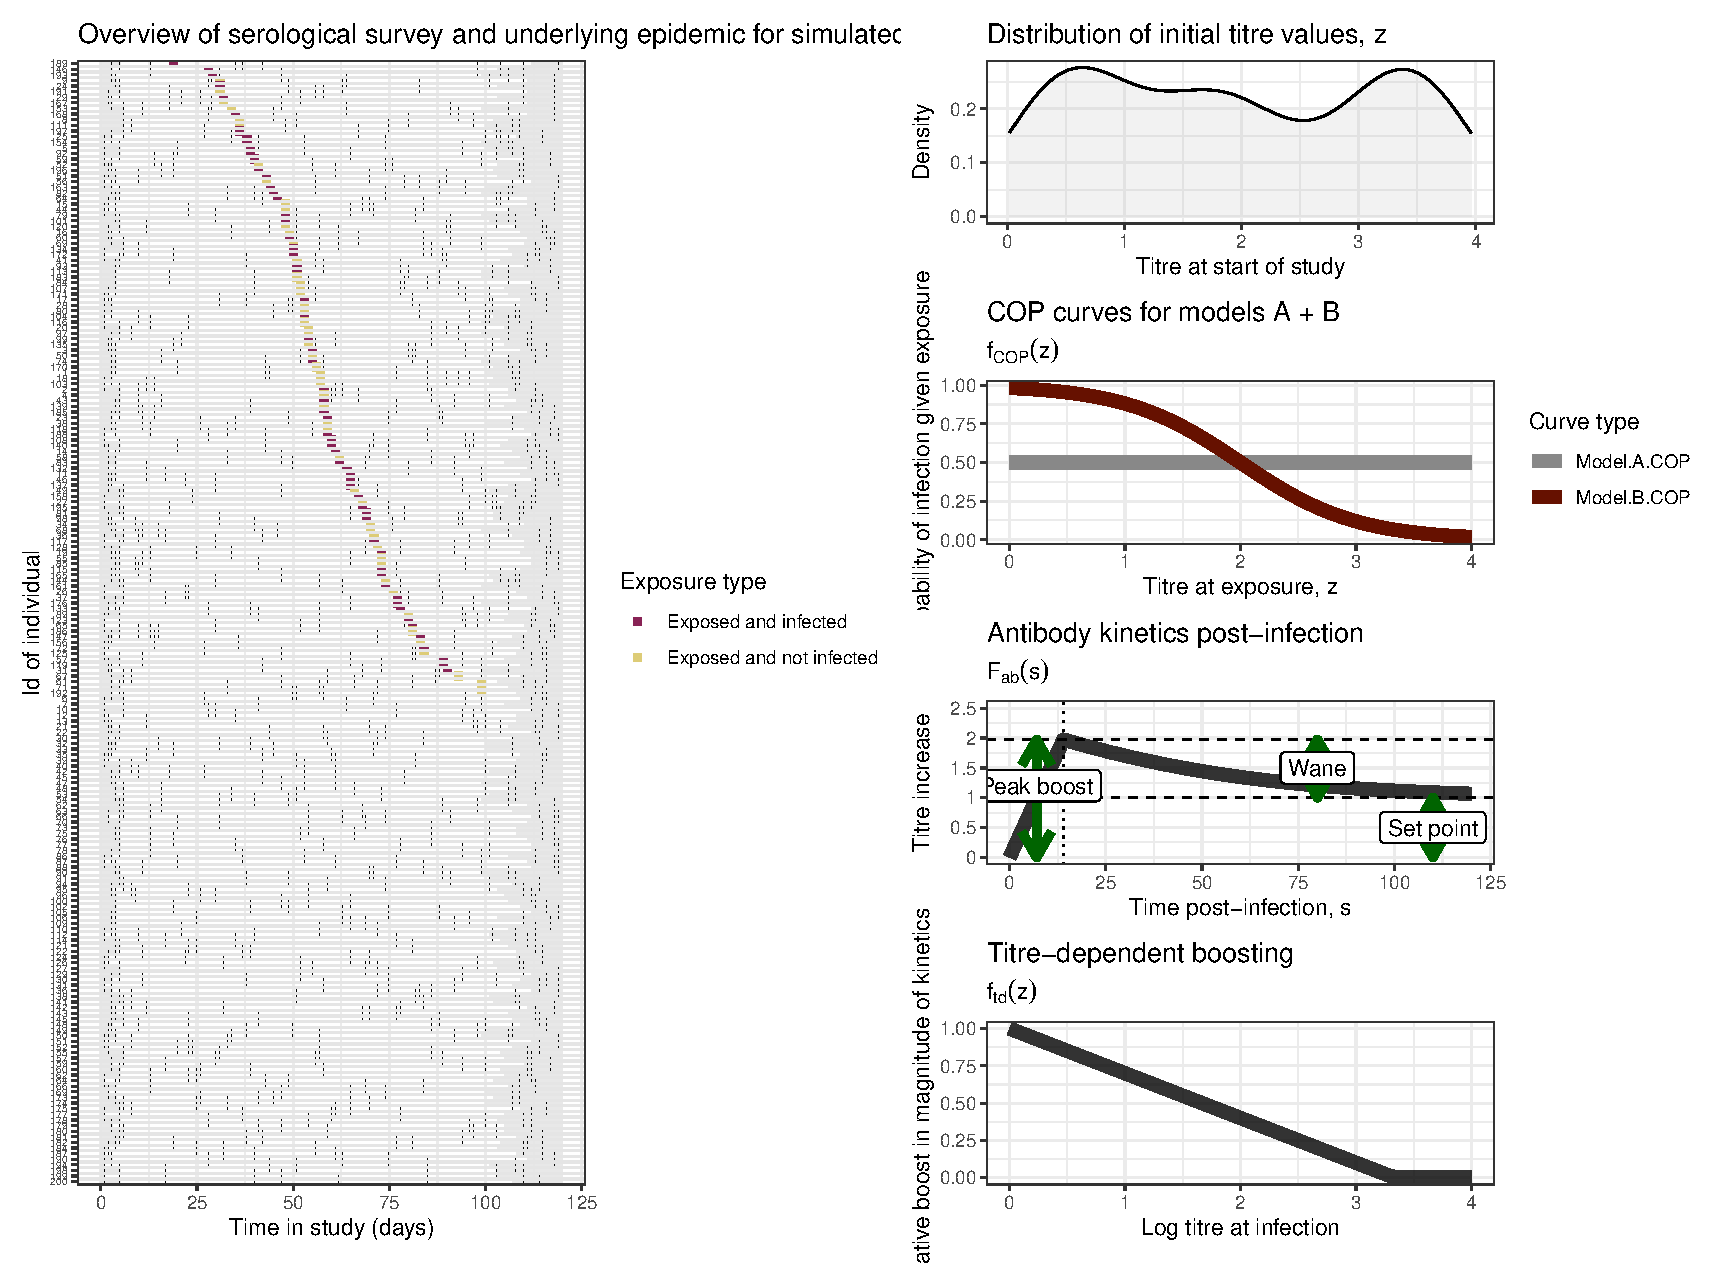
\includegraphics[width=1\textwidth]{\myimagepath/outputs/sim_data/summary_fig_A_CES.pdf}     \caption{Schematics showing the simulated data structure from \texttt{serosim}[ref]}
    \label{fig:sim_A}
\end{figure}

\paragraph{}To demonstrate the effectiveness of our modelling framework, we simulate serological data using the \texttt{serosim}[ref] R package to demonstrate its capabilities at simulation recovery. We simulate continuous epidemic serosurveillence (CES) cohort data, which represents a study in which individuals are followed over a period spanning an epidemic wave and bled at multiple random time points throughout. The simulated data includes $ M = 200$ individuals with serological samples taken within the first seven days of the study's starting and a sample within the last seven days of the study's ending. These individuals also had three samples taken randomly throughout the study (over the 120-day epidemic wave). Each individual has a 60\% chance of exposure to the virus over the study timeframe and can have a maximum of one exposure. To model an even epidemic peak, we simulate the exposure time for each individual from a normal distribution, $N(60, 20)$ days.% A figure showing the timing of the bleeds, infections and exposures for each individual is given in Figure ~\ref{fig:sim_A}.

\paragraph{}We define a correlate of protection as the probability of infection given a titre value at exposure. Two sets of data are simulated with two different correlates of protection; one is uniform at 50\% for all titres at exposure (COP model A) and thus represents no titre-dependent protection correlation. The second follows a logistic distribution (COP model B) of the form:

\begin{equation}
\label{eq_cop}
f_{cop}(x, \beta_0, \beta_1) = \frac{1}{1 + \exp(- (\beta_0 + \beta_1x))}
\end{equation}

where $\beta_0 = 2$ and $\beta_1 = 2$ in the simulated data and $x$ is the titre value at exposure. This represents a pathogen for which higher antibody titres are associated with higher levels of protection from infection. Note in this data we assume antibody trajectories remain constant until the timing of infection, such $f_{cop}(X_{j, t}, \beta_0, \beta_1) = f_{cop}(Z^0_{j}, \beta_0, \beta_1)$ where $Z^0_{j}$ is the antibody titre of an individual at their first bleed at the start of the study.

\paragraph{}Following infection, the antibody kinetics are assumed to follow a linear rise to a peak at 14 days, followed by an exponential decay to a set-point value as defined in X[ref]. The formula for this biphasic trajectory is given by Equation~\ref{eq_ab}.

\begin{equation}
\label{eq_ab}
f^1_{ab}(s, a, b, c) =
\begin{cases}
  \ln(\exp(a) + \exp(b)) / 14, & \text{if }s \leq 14 \\
  \ln(\exp(a) \exp(-(b/10)(t - 14)) + \exp(c)), &\text{if } s > 14
\end{cases}
\end{equation}

where $a = 1.5$, $b = 2$, and $c = 1$ are values in the simulated data (Figure) and $s$ is the number of days post infection. We also assume that the magnitude of these dynamics depends on pre-existing titre values, with higher pre-existing values seeing attenuated dynamics relative to lower pre-existing tire values. The titre dependent boosting is assumed to follow a linear decay truncated at 0, that is, given a titre value $z$, $f^2_{ab}(Z_j^0, \alpha) = \max(1 - \alpha z, 0)$. where $\alpha = 0.3$ in the simulated data. Therefore, the model estimated titre value at time $t$ for individual $j$, given time $s$ since infection with a titre value at infection of $Z_{j}^0$, is given by;  

\begin{equation}
\label{eq_ab2}
f_{ab}(s, Z^0_{j}, a, b, c, \alpha) = f^1_{ab}(s, a, b, c)f^2_{ab}(Z^0_{j}, \alpha) 
\end{equation}


\begin{figure}[h]
    \centering
    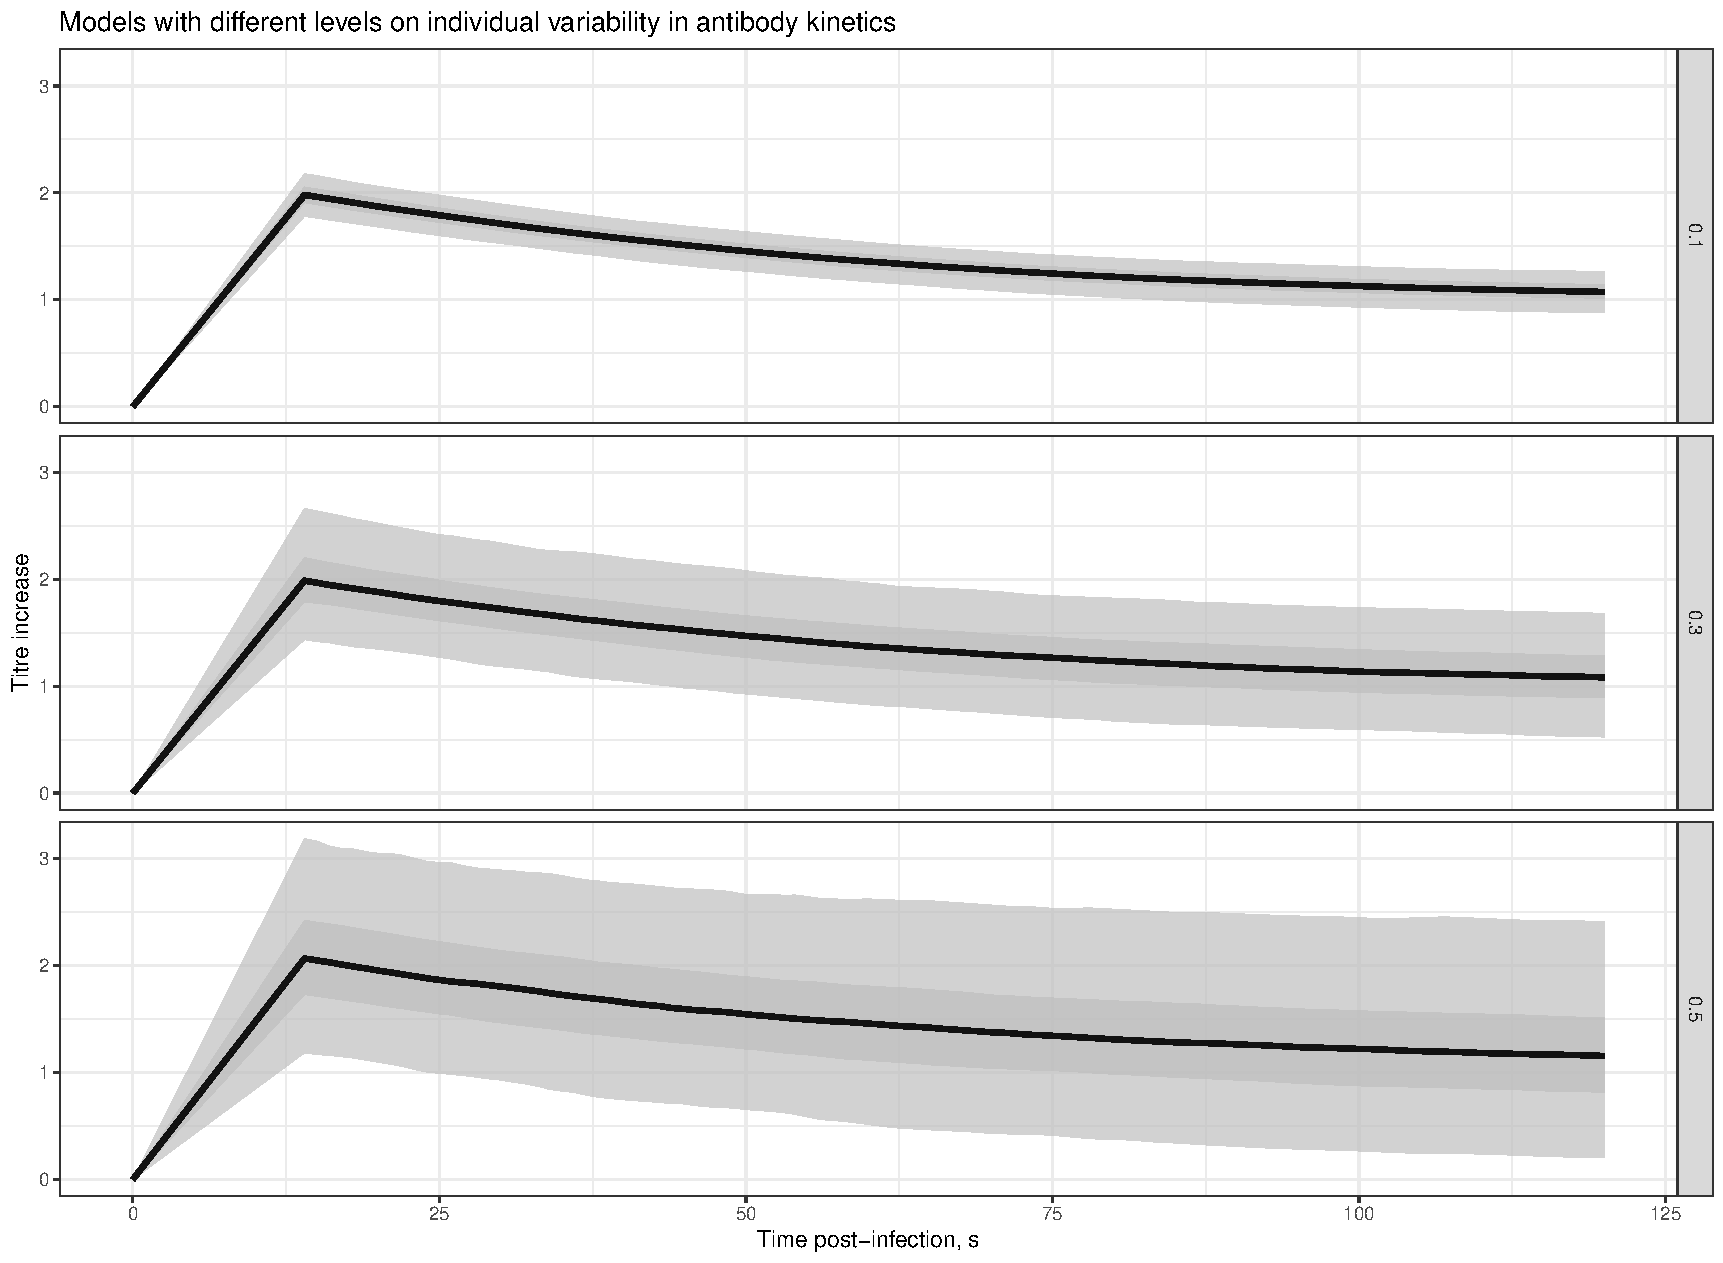
\includegraphics[width=1\textwidth]{\myimagepath/outputs/sim_data/summary_fig_B_CES.pdf}     \caption{Schematics showing three levels of individual-level uncertainty and the impact on the variability of antibody kinetics.   }
    \label{fig:sim_B}
\end{figure}



\paragraph{}To model heterogeneity in individual-level antibody kinetics, we simulate $a, b, c$, and $\alpha$ from normal distributions where the mean $\mu$ is their simulated values and the standard deviation given by $\mu\sigma^*$. We simulate three levels of uncertainty for $\sigma^* = \{0.1, 0.3, 0.5\}$, for both of the COP models, giving six simulated datasets in total. A schematic showing how these levels of uncertainty influence the variability of the antibody kinetics trajectories is shown in Figure~\ref{fig:sim_B}. We will fit the to-be-described methods to these datasets and explore how the correlation of protection and level of variability in antibody kinetics impacts the framework's ability to recover simulated data. 



We note that the simulated data for the correlate of the protection doesn't not exact match the functional form chosen when it is inferred from the infected population~\ref{}

\begin{figure}[h]
    \centering
    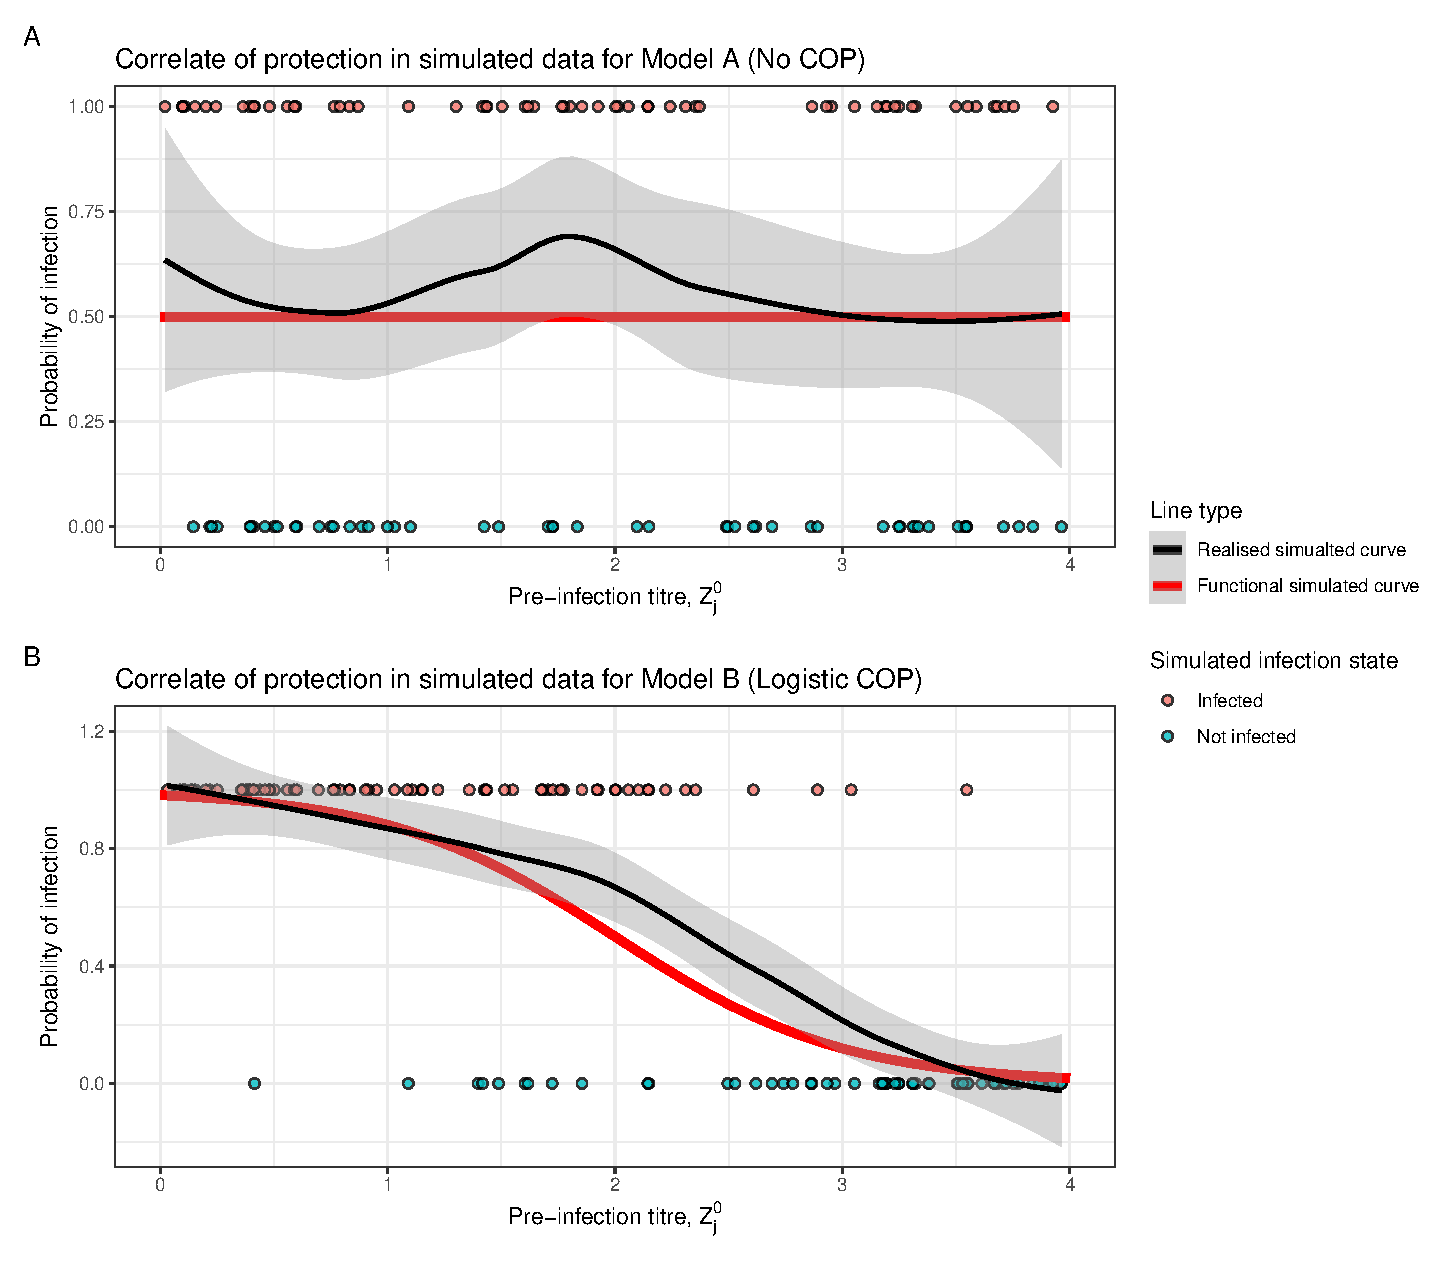
\includegraphics[width=1\textwidth]{\myimagepath/outputs/sim_data/summary_fig_C_CES.pdf}     \caption{Schematics showing the difference between the functional form chosen to simulate the COP and the recovered COP from the exposed individuals.   }
    \label{fig:sim_C}
\end{figure}


